\begin{figure}
\begin{center}
\tikzset{every picture/.style={line width=0.75pt}} %set default line width to 0.75pt        
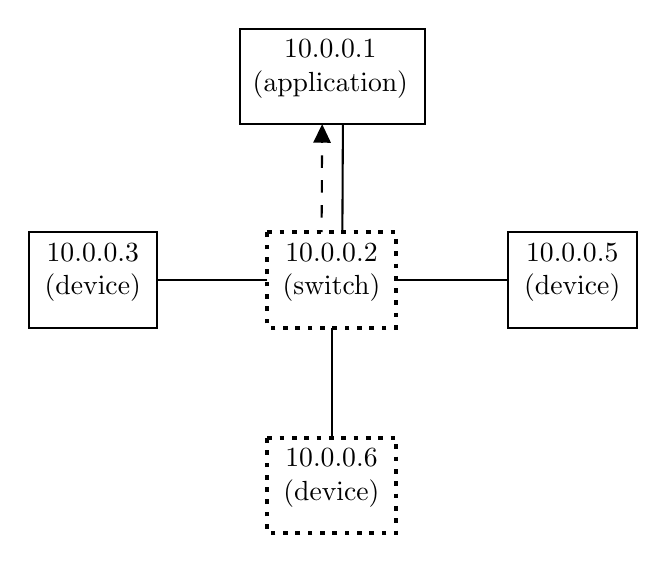
\begin{tikzpicture}[x=0.75pt,y=0.75pt,yscale=-1,xscale=1]
    %uncomment if require: \path (0,278); %set diagram left start at 0, and has height of 278
    % Text Node
    \draw    (122,17) -- (211,17) -- (211,63) -- (122,63) -- cycle  ;
    \draw (125,21) node [anchor=north west][inner sep=0.75pt]   [align=left] {\begin{minipage}[lt]{58.25pt}\setlength\topsep{0pt}
    \begin{center}
    10.0.0.1\\(application)
    \end{center}

    \end{minipage}};
    % Text Node
    \draw  [dash pattern={on 1.69pt off 2.76pt}][line width=1.5]   (135,115) -- (197,115) -- (197,161) -- (135,161) -- cycle  ;
    \draw (138,119) node [anchor=north west][inner sep=0.75pt]   [align=left] {\begin{minipage}[lt]{39.55pt}\setlength\topsep{0pt}
    \begin{center}
    10.0.0.2\\(switch)
    \end{center}

    \end{minipage}};
    % Text Node
    \draw    (20,115) -- (82,115) -- (82,161) -- (20,161) -- cycle  ;
    \draw (23,119) node [anchor=north west][inner sep=0.75pt]   [align=left] {\begin{minipage}[lt]{39.55pt}\setlength\topsep{0pt}
    \begin{center}
    10.0.0.3\\(device)
    \end{center}

    \end{minipage}};
    % Text Node
    \draw  [dash pattern={on 1.69pt off 2.76pt}][line width=1.5]   (135,214) -- (197,214) -- (197,260) -- (135,260) -- cycle  ;
    \draw (138,218) node [anchor=north west][inner sep=0.75pt]   [align=left] {\begin{minipage}[lt]{39.55pt}\setlength\topsep{0pt}
    \begin{center}
    10.0.0.6\\(device)
    \end{center}

    \end{minipage}};
    % Text Node
    \draw    (251,115) -- (313,115) -- (313,161) -- (251,161) -- cycle  ;
    \draw (254,119) node [anchor=north west][inner sep=0.75pt]   [align=left] {\begin{minipage}[lt]{39.55pt}\setlength\topsep{0pt}
    \begin{center}
    10.0.0.5\\(device)
    \end{center}

    \end{minipage}};
    % Connection
    \draw    (171.38,63) -- (171.12,115) ;
    % Connection
    \draw    (197,138) -- (251,138) ;
    % Connection
    \draw    (135,138) -- (82,138) ;
    % Connection
    \draw  [dash pattern={on 4.5pt off 4.5pt}]  (161.37,66) -- (161.12,115) ;
    \draw [shift={(161.38,63)}, rotate = 90.29] [fill={rgb, 255:red, 0; green, 0; blue, 0 }  ][line width=0.08]  [draw opacity=0] (8.93,-4.29) -- (0,0) -- (8.93,4.29) -- cycle    ;
    % Connection
    \draw    (166,161) -- (166,214) ;

\end{tikzpicture}
\end{center}
\caption{Communication is marked as an arrow, scanned devices are highlighted.}
\label{Figure:NetworkDeviceAdded}
\end{figure}